\documentclass[12pt,a4paper]{book}
\usepackage{setspace}
%\doublespace %para doble espacio
\onehalfspace
\usepackage{caption}

\usepackage[utf8]{inputenc}
\usepackage[spanish]{babel}
\usepackage{latexsym}

\usepackage{amsfonts}
\usepackage[leqno]{amsmath}
\usepackage{rotating}
\usepackage{url}
\usepackage{proof}
\usepackage{alltt}
\usepackage{hyperref}
\usepackage{verbatim}
\usepackage{amssymb}

\usepackage{graphicx}
\usepackage[usenames]{color}
\usepackage{psfrag}
\usepackage{xypic}
\usepackage{proof}
\usepackage{indentfirst}
\usepackage[verbose]{geometry}
\usepackage{appendix}
\usepackage{tabulary} 
\usepackage[acronym,nonumberlist,shortcuts,sanitize=none,nomain]{glossaries}

\geometry{a4paper}
\geometry{top=3cm,bottom=3cm,left=3cm,right=3cm,headsep=1cm}

% Punto decimal spanish
\makeatletter
\def\es@decimal{{.}}
\makeatother


\usepackage{pdfpages}
\usepackage{fancyhdr}
\renewcommand{\labelitemi}{\leavevmode\hbox to 1.2ex
      {\hss\vrule height .9ex width .7ex depth -.2ex\hss}}
\pagestyle{fancy}
  \renewcommand{\headrulewidth}{0pt}

\renewcommand{\chaptermark}[1]{\markboth{\chaptername\ \thechapter.\ #1}{}}
\renewcommand{\sectionmark}[1]{\markright{\thesection.\ #1}}

\fancyhf{}
\fancyhead[LO]{\textsc{\rightmark}}
\fancyhead[RE]{\textsc{\leftmark}}
\fancyhead[RO,LE]{\thepage}
\fancyfoot[LE,RO]{}
\fancypagestyle{plain}{%
  \fancyhf{}  
  \fancyfoot[C]{\thepage}
  \renewcommand{\headrulewidth}{0pt}
}


 \newtheorem{prop}{Proposition}[section]
 \newtheorem{theo}{Theorem}[section]
 \newtheorem{lemma}{Lemma}[section]
 \newtheorem{constr}{Construction}[section]
 \newtheorem{defin}{Definition}[section]
 \newtheorem{ex}{Example}[section]
 \newtheorem{alg}{Algorithm}[section]
      \newtheorem{cor}{Corollary}[section]
 \newtheorem{pro}{Problem}[section]
\newtheorem{COROLLARY}{\indent Corollary}
\newenvironment{corollary}[1]
{\begin{COROLLARY}\fullstop\label{#1}\sl}{\rm\end{COROLLARY}}
\newtheorem{EXAMPLE}{\indent Example}
\newenvironment{example}[1]
{\begin{EXAMPLE}\fullstop\label{#1}\rm}{\rm\end{EXAMPLE}}
\newtheorem{THEOREM}{\indent Theorem}
\newenvironment{theorem}[1]
{\begin{THEOREM}\fullstop\label{#1}\sl}{\rm\end{THEOREM}}
\newtheorem{REMARK}{\indent Remark}
\newenvironment{remark}[1]
{\begin{REMARK}\fullstop\label{#1}\rm}{\rm\end{REMARK}}
\newcommand{\bldu}{{\bf u}}
\newcommand{\bldv}{{\bf v}}
\newcommand{\bldy}{{\bf y}}
\newcommand{\ontopof}[2]{{{\scriptstyle{#1}} \atop {\scriptstyle{#2}}}}
\newcommand{\Eq}[1]{(\ref{#1})}
\newcommand{\bldalpha}{\mbox{\boldmath $\alpha$}}
\newcommand{\be}{\mbox{$\beta$}}
\newcommand{\clauseend}{\hspace*{\fill}\mbox{$\bullet$}}
\newcommand{\fullstop}{\hspace{-0.85em} {\bf .}}
\newcommand{\bldc}{{\bf c}}
\newcommand{\deff}{\stackrel{\Delta}{=}}
\newcommand{\ur}{\mbox{$\underline{r}$}}
\newcommand{\ua}{\mbox{$\underline{a}$}}
\newcommand{\ub}{\mbox{$\underline{b}$}}
\newcommand{\uh}{\mbox{$\underline{h}$}}
\newcommand{\uv}{\mbox{$\underline{v}$}}
\newcommand{\ue}{\mbox{$\underline{e}$}}
\newcommand{\us}{\mbox{$\underline{s}$}}
\newcommand{\uu}{\mbox{$\underline{u}$}}
\newcommand{\uy}{\mbox{$\underline{y}$}}
\newcommand{\ux}{\mbox{$\underline{x}$}}
\newcommand{\uc}{\mbox{$\underline{c}$}}
\newcommand{\ud}{\mbox{$\underline{d}$}}
\newcommand{\ut}{\mbox{$\underline{t}$}}
\newcommand{\ug}{\mbox{$\underline{g}$}}
\newcommand{\hX}{\mbox{$\hat{X}$}}
\newcommand{\hY}{\mbox{$\hat{Y}$}}
\newcommand{\hZ}{\mbox{$\hat{Z}$}}
\newcommand{\hs}{\mbox{$\hat{s}$}}
\newcommand{\hS}{\mbox{$\hat{S}$}}
\newcommand{\ra}{\mbox{$\rightarrow$}}
\newcommand{\Ra}{\mbox{$\Rightarrow$}}
\newcommand{\La}{\mbox{$\Leftarrow$}}
\newcommand{\la}{\mbox{$\leftarrow$}}
\newcommand{\lra}{\mbox{$\leftrightarrow$}}
\newcommand{\lam}{\mbox{$\lambda$}}
\newcommand{\al}{\mbox{$\alpha$}}
%\newcommand{\r}{\mbox{$\rho$}}
\newcommand{\si}{\mbox{$\sigma$}}
\newcommand{\eq}{\mbox{$\, =\,$}}
\newcommand{\om}{\mbox{$\omega$}}
\newcommand{\lan}{\mbox{$\langle$}}
\newcommand{\ran}{\mbox{$\rangle$}}
\newcommand{\lf}{\mbox{$\lfloor$}}
\newcommand{\rf}{\mbox{$\rfloor$}}
\newcommand{\lc}{\mbox{$\lceil$}}
\newcommand{\rc}{\mbox{$\rceil$}}
\newcommand{\ap}{\mbox{$\approx$}}
\newcommand{\qed}{\hfill$\Box$\\[1ex]}
\newcommand{\pf}{{\bf Proof: }}
\newcommand{\pr}{\vspace{.8cm} {\bf Problems}}
\newcommand{\uw}{\mbox{$\underline{w}$}}
\newcommand{\uell}{\mbox{$\underline{\ell}$}}
\newcommand{\uzero}{\mbox{$\underline{0}$}}
\newcommand{\uone}{\mbox{$\underline{1}$}}
\newcommand{\xor}{\mbox{$\oplus$}}
\newcommand{\lcm}{\mbox{${\rm lcm}$}}
\newcommand{\C}{\mbox{${\cal C}$}}
\newcommand{\B}{\mbox{${\cal B}$}}
\newcommand{\hU}{\mbox{${\hat{U}}$}}
\newcommand{\hV}{\mbox{${\hat{V}}$}}
\newcommand{\hW}{\mbox{${\hat{W}}$}}
\newcommand{\hA}{\mbox{${\hat{A}}$}}
\newcommand{\s}{\mbox{${\cal S}$}}
\newcommand{\A}{\mbox{${\cal A}$}}
\newcommand{\EO}{\mbox{${\cal EO}$}}
\newcommand{\E}{\mbox{${\cal E}$}}
\newcommand{\R}{\mbox{${\cal R}$}}
\newcommand{\G}{\mbox{${\cal G}$}}
\newcommand{\cC}{\mbox{${\cal C}$}}
\newcommand{\cO}{\mbox{${\cal O}$}}
\newcommand{\rg}{\mbox{$\overrightarrow{g}$}}
\newcommand{\lag}{\mbox{$\overleftarrow{g}$}}
\newcommand{\dummy}{\mbox{$\,$}}
\newcommand{\bp}{\newpage}
\newcommand{\br}{\\ }
\newcommand{\ce}{\begin{center}}
\newcommand{\cen}{\end{center}}
\newcommand{\fB}{\bf}
\newcommand{\fI}{\it}
\newcommand{\fR}{\rm}
\newcommand{\hl}{\dummy\hrulefill\dummy}
\newcommand{\ip}[1]{\item[{\rm {#1}}]}
\newcommand{\ipb}{\begin{description}}
\newcommand{\ipn}{\end{description}}
\newcommand{\lp}{\par\noindent}
\newcommand{\bld}[1]{{\bf {#1}}}
\newcommand{\itl}[1]{{\it {#1}}}
\newcommand{\rmn}[1]{{\rm {#1}}}
\newcommand{\pp}{\par}
\newcommand{\qb}{\begin{quote}}
\newcommand{\qn}{\end{quote}}
\newcommand{\sh}[2]{\section{\Pd #1}\label{#2}}
\newcommand{\spc}[1]{\vspace{#1}}
\newcommand{\tp}{\begin{titlepage}}
\newcommand{\tpn}{\end{titlepage}}
\newcommand{\zb}{\begin{figure}[hbtp]}
\newcommand{\zn}{\end{figure}}
\newcommand{\EQ}{\[}
\newcommand{\EN}{\]}
\newcommand{\EQX}[1]{\begin{equation}\label{#1}}
\newcommand{\ENX}{\end{equation}}
\newcommand{\EQL}{\begin{eqnarray*}}
\newcommand{\ENL}{\end{eqnarray*}}
\newcommand{\EQLX}[1]{\begin{eqnarray}\label{#1}}
\newcommand{\ENLX}{\end{eqnarray}}
\newcommand{\Pd}{\hspace{-1.35em}
           {\bf .} \hspace {0.35em}}
\newcommand{\lpsh}{\nopagebreak\par\noindent\nopagebreak}
\newcommand{\ppsh}{\nopagebreak\par\nopagebreak}
\newcommand{\open}{\begin{document}}
\newcommand{\close}{\end{document}}
\newcommand{\lfcr}[1]{\br\hspace*{#1em}}
\newenvironment{mat}[1]
{\left[\begin{array}{#1}}{\end{array}\right]}
\newcommand{\GAMMA}{\Gamma}
\newcommand{\DELTA}{\Delta}
\newcommand{\THETA}{\Theta}
\newcommand{\LAMBDA}{\Lambda}
\newcommand{\XI}{\Xi}
\newcommand{\PI}{\Pi}
\newcommand{\SIGMA}{\Sigma}
\newcommand{\UPSILON}{\Upsilon}
\newcommand{\PHI}{\Phi}
\newcommand{\PSI}{\Psi}
\newcommand{\OMEGA}{\Omega}
\newcommand{\bldgreek}[1]{\mbox{\boldmath $#1$}}
\newcommand{\bldbeta}{\bldgreek{\beta}}
\newcommand{\bldgamma}{\bldgreek{\gamma}}
\newcommand{\blddelta}{\bldgreek{\delta}}
\newcommand{\bldepsilon}{\bldgreek{\epsilon}}
\newcommand{\bldvarepsilon}{\bldgreek{\varepsilon}}
\newcommand{\bldzeta}{\bldgreek{\zeta}}
\newcommand{\bldeta}{\bldgreek{\eta}}
\newcommand{\bldtheta}{\bldgreek{\theta}}
\newcommand{\bldvartheta}{\bldgreek{\vartheta}}
\newcommand{\bldiota}{\bldgreek{\iota}}
\newcommand{\bldkappa}{\bldgreek{\kappa}}
\newcommand{\bldlambda}{\bldgreek{\lambda}}
\newcommand{\bldmu}{\bldgreek{\mu}}
\newcommand{\bldnu}{\bldgreek{\nu}}
\newcommand{\bldxi}{\bldgreek{\xi}}
\newcommand{\bldpi}{\bldgreek{\pi}}
\newcommand{\bldvarpi}{\bldgreek{\varpi}}
\newcommand{\bldrho}{\bldgreek{\rho}}
\newcommand{\bldvarrho}{\bldgreek{\varrho}}
\newcommand{\bldsigma}{\bldgreek{\sigma}}
\newcommand{\bldvarsigma}{\bldgreek{\varsigma}}
\newcommand{\bldtau}{\bldgreek{\tau}}
\newcommand{\bldupsilon}{\bldgreek{\upsilon}}
\newcommand{\bldphi}{\bldgreek{\phi}}
\newcommand{\bldvarphi}{\bldgreek{\varphi}}
\newcommand{\bldchi}{\bldgreek{\chi}}
\newcommand{\bldpsi}{\bldgreek{\psi}}
\newcommand{\bldomega}{\bldgreek{\omega}}
\addto\extrasspanish{\def\tablename{Tabla}}



\graphicspath{{figuras/}}
\begin{document}

\thispagestyle{empty}

\begin{frontmatter}
\thispagestyle{empty}

\begin{huge}
\mbox{ }
\vfill
\newlength{\longTitulo}
%\settowidth{\longTitulo}{%
%\textbf{L\'inea 1 T\'itulo}}
\begin{center}
\rule{135mm}{.5mm}\\
\vskip .3cm
\textbf{Identificación de la fuente de adquisición de imágenes/vídeos en escenarios abiertos usando técnicas de IA}\\
\rule{135mm}{.5mm}\\
\end{center}
\end{huge}

\vfill


  \begin{center}
				{\scalebox{.3}{
\includegraphics{LogoUCM}}}
  \end{center}

\vfill

\begin{center}
  {\Large {\bf IMPLANTACIÓN CORPORATIVA DE TECNOLOGÍAS, SERVICIOS Y SISTEMAS INFORMÁTICOS}}
\end{center}
\begin{center}
Máster en Ingeniería Informática
\end{center}

%\begin{center}
  %{\Large {\bf CURSO 2012-2013}}
%\end{center}

\vfill


\begin{large}
\begin{center}
\begin{Large}
  	{\bf Ignacio Gago Padreny}
\end{Large}
%\vfill
%\vskip .7cm
  \\ \mbox{ } \\ \mbox{ } \\ 
%{\it Directores}  \\ [0.3em]
  %{\bf  Luis Javier Garc\'ia Villalba, Ana Lucila Sandoval Orozco}
  \vspace{.5ex}
\begin{large}
\begin{center}
\vskip .5cm
%{\bf Calificaci\'on: SOBRESALIENTE}
\vfill
\vspace{3ex}
%\text{Departamento de Ingenier\'ia del Software e Inteligencia Artificial}\\[0.2em]
\text{Facultad de Inform\'atica}\\[0.2em]
\text{Universidad Complutense de Madrid}\\[1em]
\text{Madrid, Junio de 2016}
\end{center}
\end{large}
\end{center}

\vfill

\end{large}

\newpage
\thispagestyle{empty}
\mbox{ }


\clearpage
\pagestyle{fancy}
\fancyhf{}
\fancyhead[LO]{\textsc{\rightmark}}
\fancyhead[RE]{\textsc{\leftmark}}
\fancyhead[RO,LE]{\thepage}
\fancyfoot[LE,RO]{}%\vspace*{1cm}\small \sc Borrador \today}
\fancypagestyle{plain}{%
  \fancyhf{}  
  \fancyfoot[C]{\thepage}
  \renewcommand{\headrulewidth}{0pt}
}


%%%%%%%%%%%%%%%%%%%%%%%%%%%%%%%%%%%%%%%%%%%%%%%%%%%%%%%%%%
%

%\newpage
%\mbox{}\vfill

\end{frontmatter}


%\begin{otherlanguage}{spanish}

%\thispagestyle{empty}
%\section*{Agradecimientos}
%\input{agradecimientos}
%\end{otherlanguage}

%\newpage
%\thispagestyle{empty}
%\mbox{ }

%\newpage
%\thispagestyle{empty}
%\section*{Abstract}
%\input{abstract}

%\newpage
%\thispagestyle{empty}
%\mbox{ }

%\newpage

%\begin{otherlanguage}{spanish}
%\thispagestyle{empty}
%\section*{Resumen}
%\input{resumen}
%\end{otherlanguage}

%\newpage
%\thispagestyle{empty}
%\mbox{ }

%\newpage
%\thispagestyle{empty}
%\input{autorizacion}

%\newpage
%\thispagestyle{empty}
%\mbox{ }
% hoja en blanco
%\newpage
%\thispagestyle{empty}


\begin{otherlanguage}{spanish}
\pagestyle{empty}

\renewcommand{\contentsname}{\'Indice General} \thispagestyle{empty}
\renewcommand{\listtablename}{\'Indice de Tablas} \thispagestyle{empty}
\renewcommand{\listfigurename}{\'Indice de Figuras}  \thispagestyle{empty}
\renewcommand{\appendixname}{Ap\'endices} \thispagestyle{empty}
\renewcommand{\appendixtocname}{Ap\'endices} \thispagestyle{empty}
\renewcommand{\appendixpagename}{Ap\'endices} \thispagestyle{empty}

%\begin{comment}
%acronimos
%\setlength{\glslistdottedwidth}{.4\linewidth}
%\setlength{\glslistdottedwidth}{3cm}
%\setlength{\glsdescwidth}{10cm}
%\printglossary[type=acronym, style=long]
%\parindent=0cm
%\renewcommand*{\glsgroupskip}{}
%\glsgroupskip
%\printglossary[type=acronym, style=listdotted]
%\addcontentsline{toc}{chapter}{Lista de Acr\'onimos}
%\input{acronimos} 
%\end{comment}
 
%acronimos
%\pagestyle{fancy}
%\section*{Lista de Acr\'onimos}
%\input{acronimos}

\pagenumbering{gobble}
\tableofcontents
%\listoftables
%\listoffigures

%\chapter{Objetivos de este trabajo}
%\pagestyle{plain}
%\pagenumbering{arabic}
%El campo de la ciberseguridad informática ha tomado especial interés en los últimos a\~nos, convirtiéndose en una fuente de estudio para muchos investigadores. El objetivo de este trabajo es el estudio de los ataques de denegación de servicio, tanto sus métodos como sus defensas, debido a la gran relevancia que tienen estos dentro del campo de la ciberseguridad. 


\chapter{Vídeos Digitales}
\pagestyle{plain}
\pagenumbering{arabic}
En este capítulo se describen los principales conocimientos sobre vídeos relacionados con el objetivo principal de este trabajo. En primer lugar se detalla el proceso de generación de un vídeo y su composición basada en imágenes para luego hablar de los métodos más habituales de compresión para el almacenamiento del mismo. Una vez explicado este proceso se comentará cómo interviene el tipo de sensor en la extracción del ruido del dispositivo.

\section{Proceso de generación de un vídeo digital}
El proceso de generación de un vídeo digital está basado en transformar se\~nales analógicas (funciones con dominio continuo y que toman valores en un conjunto continuo) en se\~nales digitales, capaces de ser procesadas por un ordenador. Para convertir una se\~nal analógica en una se\~nal digital (conversión A/D) se utilizan dos técnicas: muestreo y cuantificación.
\subsection{Muestreo}
El proceso de muestreo o \textit{sampling} consiste en transformar una se\~nal con dominio continuo en otra de dominio discreto, de forma que se retenga el máximo posible de la información original de la se\~nal analógica. Gráficamente se puede ver un ejemplo de muestreo en \ref{fig_muestreo}.

\begin{figure}[ht!]
\begin{center}
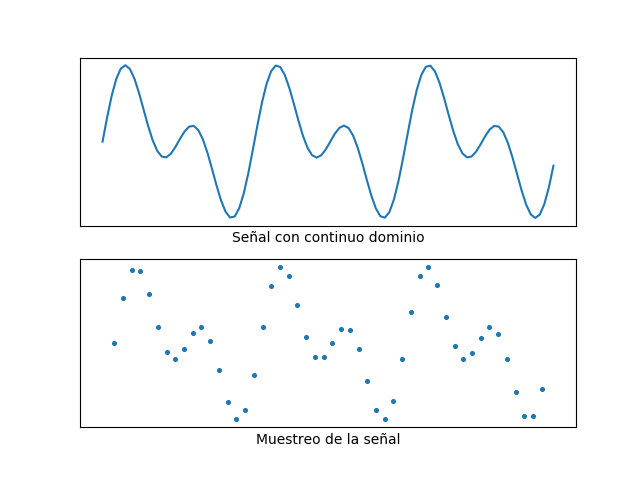
\includegraphics{figuras/muestreo.png}
\end{center}
\caption{Muestro de una se\~nal de dominio continuo}
\label{fig_muestreo}
\end{figure}

La técnica del muestreo ha sido ampliamente estudiada pues es usada en una gran variedad de campos y existen métodos y fórmulas matemáticas para determinar cotas inferiores que no elimenen información del original, sin embargo en este contexto hay cotas menos exigentes debido a la capacidad que tiene el cerebro para procesar visualmente un objeto. 
En el contexto de este trabajo hay dos tipos diferentes que se deben realizar: uno asociado a las variables espaciales y otro asociado al tiempo. Ambos casos se basan en tener muestras muy cercanas de forma que la composición parezca continua y no discreta.
El muestro de la variable temporal está relacionado con el número de imágenes por segundo que es capaz de procesar el ojo humano, estando entre 25 y 30 lo que el ojo ya percibe como continuo.
Al discretizar la sen\~al analógica obtenemos un conjunto finito que podemos numerar y expresar en forma de una matriz de dos dimensiones, siendo cada una de las celdas un pixel (del inglés \textit{picture element}). Para el número de filas y columnas elegido por el muestro se toma un múltiplo de dos, puesto que tiene por una parte la ventaja de favorecer el direccionamiento de las muestras y por otra de ser más eficientes para ciertos algoritmos como puede ser la transformada de Fourier.
En el muestro también interviene la frecuencia de la se\~nal original: una con baja frecuencia puede ser bien representada con una tasa de muestreo determinada, pero la misma puede ser no válida para una frecuencia alta, produciéndose el efecto que conocemos como solapamiento o \textit{aliasing}. El teorema de Nyquist establece que utilizando una tasa de muestro mayor al doble de la frecuencia original, se evita el \textit{aliasing} y se puede recuperar la se\~nal original a partir de la transformada. En \ref{fig_nyquist} se puede observar como cuando la frecuencia de muestreo es suficientemente grande comparado con la frecuencia original (figura de arriba) se puede reconstruir la onda original, mientras que en la figura de abajo se observa que cuando no se cumple el Teorema de Nyquist se produce una pérdida de información que impide reconstruir la se\~nal original\cite{b3:2012}.

\begin{figure}[ht!]
\begin{center}
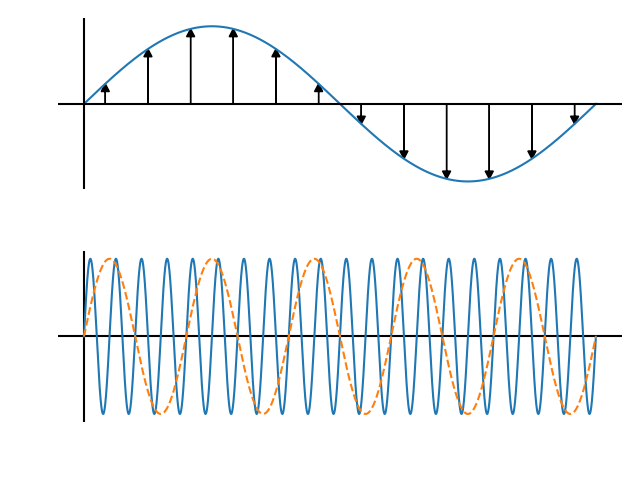
\includegraphics{figuras/nyquist.png}
\end{center}
\caption{Frecuencia en el muestreo}
\label{fig_nyquist}
\end{figure}

\subsection{Cuantificación}
La cuantificación consiste en transformar el rango continuo de la se\~nal analógica en un rango discreto. La intensidad que es una se\~nal continua es transformada a un conjunto finito que son los valores que pueden tomar los pixels. De esta forma, mientras que con el muestro reducimos una variable espacial continua en una matrix, la cuantificación permite que la intensidad que capta la lente del dispostivo se pueda representar por un conjunto discreto de valores. 
De la misma forma que en el muestreo, se suele utilizar un conjunto de cardinalidad potencia de dos. Para imágenes en color lo usual es trabajar con tres componentes cada uno de ocho bits, mientras que en las imágenes en blanco y negro se trabaja con un componente de ocho bits. 
Cabe destacar que este proceso no es reversible y está asociado a funciones no lineares, al contrario que el muestro, en el que partiendo de premisas no muy exigentes se puede reconstruir la se\~nal analógica. \\

El proceso de cuantificación en vídeo se basa en aplicar frame a frame el método que se aplica en JPEG. En primer lugar se divide la imagen o frame en bloques disjuntos de $8$x$8$ pixels, para cada uno de estos bloques $B$ se calcula la transformada del coseno discreta (DCT) siguiendo\cite{fridrich:2003}:

\begin{equation}
D_{ij} = \sum_{k,l=0}^{7}a_{kl}(i,j)B_{kl} \nonumber
\end{equation}

donde
\begin{equation} \label{eq:dct}
a_{kl}(i,j) = \frac{1}{4}w(k)w(l)\cos\frac{\pi}{16}k(2i+1)\cos\frac{\pi}{16}k(2j+1) 
\end{equation}

y

\begin{equation}
w(k) = 
\begin{cases}
\frac{\displaystyle 1}{\displaystyle\sqrt{2}} & \text{si $k=0$}\\
1 & \text{en caso contrario} \nonumber
\end{cases}
\end{equation}

Aplicando DCT se transforma la fuente original en el dominio de las frecuencias. Los coeficientes $a_{kl}$ de la ecuación \ref{eq:dct}, multiplicadores de los valores del bloque de la imagen, cumplen que a medida que nos distanciamos de la primera fila se incrementa la varianza, como podemos ver en \ref{fig_dct}. Además, a medida que nos distanciamos de la primera columna también crece la varianza. Por otra parte, los coeficientes DCT que se corresponden con frecuencias bajas son grandes en magnitud.

\begin{figure}[ht!]
\begin{center}
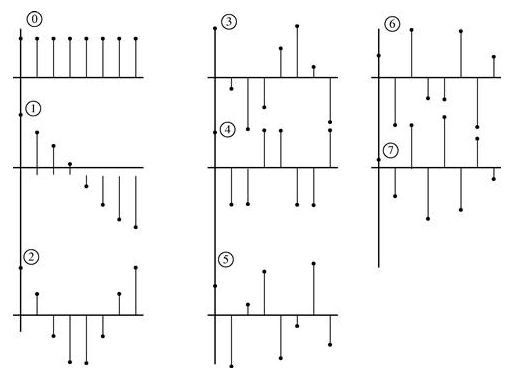
\includegraphics[width=10cm,height=10cm,keepaspectratio]{figuras/dct.png}
\end{center}
\caption{Varianza según la fila del bloque en la transformada DCT, \cite{b4:2012}}
\label{fig_dct}
\end{figure}


La matriz $D$ con los coeficientes DCT es discretizada posteriormente utilizando una matriz de cuantificación $Q$, producto de una tabla de valores y cuantificación y una escala de cuantificicación, fija en el caso de una tasa de bits variable (VBR) y variable en el caso de una tasa de bits constante (CBR). 
\begin{equation}
D_{ij} = round\left(\frac{D_{ij}}{Q_{ij}}\right),  i,j\in\{0, \dots, 7\} \nonumber
\end{equation}

En la matriz de cuantificación, cada elemento define el umbral bajo el cual un detalle en la imagen debe ser capturado como tal o descartado. De esta forma, a medida que nos alejamos del origen, ya sea horizontal o verticalmente, se exige un mayor coeficiente DCT para que el detalle sea relevante, puesto que se corresponden con valores de mayor frecuencia. Hay una gran variedad de matrices de cuantificación, calculadas normalmente en base a experimentos psico-visuales para determinar los umbrales DCT. Una matriz de cuantificación ampliamente utilizada es la siguiente\cite{b3:2012}:
$$
\begin{bmatrix}
8 & 16 & 19 & 22 & 26 & 27 & 29 & 34 \\
16 & 16 & 22 & 24 & 27 & 29 & 34 & 37 \\
19 & 22 & 26 & 27 & 29 & 34 & 34 & 38 \\
22 & 22 & 26 & 27 & 29 & 34 & 37 & 40 \\
22 & 26 & 27 & 29 & 32 & 35 & 40 & 48 \\
26 & 27 & 29 & 32 & 35 & 40 & 48 & 58 \\
26 & 27 & 29 & 34 & 38 & 46 & 56 & 69 \\
27 & 29 & 35 & 38 & 46 & 56 & 69 & 83 \\
\end{bmatrix}
$$

\section{Almacenamiento de vídeos digitales}
Del proceso descrito en la sección anterior, es fácil deducir que la cantidad de datos en se\~nales visuales es grande. Una imagen en blanco y negro de dimensiones $M$x$N$ con $B$ bits para el nivel de resolución del gris supone un tama\~no de $NMB$ bits. Esto supone que una sola imagen de color de $512$ x $512$ x $8$ ocupa cerca de 1MB. Esto implica que un vídeo con estas características y una tasa de muestro de 30 frames por segundo (el mínimo para que el ojo humano lo detecte como continuo) requiere 23.6MB por segundo\cite{b2:2005}.\\

Esta gran cantidad de datos que sería necesaria para almacenar un vídeo no solamente supone un problema en cuanto a requisitos de memoria, si no también para el procesamiento y trasmisión de los mismos. Como consecuencia, es necesario reducir la cantidad de datos mediante algoritmos de compresión, que en el caso de vídeos están definidos por el comité MPEG (del inglés \textit{Moving Pictures Expert Group}) de forma estándar e internacional.
Como ya se ha comentado anteriormente, se puede ver un vídeo como una sucesión de imágenes o \textit{frames}. Además de aprovechar la compresión de imágenes, en el caso del vídeo se tiene una redundancia temporal ya que el siguiente frame tiene mucho en común con el actual y los anteriores, factor que se aprovechará para reducir el tama\~no. \\

Los algoritmos de codificación más utilizados han sido definidos por un grupo de expertos conocido como MPEG (del inglés \textit{Motion Picture Expert Group}) y se basan, al igual que la mayoría de algoritmos de compresión de vídeo en el concepto llamado grupo de imágenes o GOP (del inglés \textit{Group Of Pictures}). Un GOP de tama\~no $N$ está compuesto de $N$ imágenes que pueden ser de tipo:
\begin{itemize}
\item Los \textbf{I-frames} o \textit{intra-coded frames} se codifican de forma independiente, sin referencias a otros frames. Esto permite acceso aleatorio a los datos del vídeo, puesto que pueden ser decodificados sin necesitar de otros frames. Además de esto, tienen la ventaja de evitar la propagación de errores que se acarrea en la compresión de frames consecutivos al contener la mayor información de la escena por si solos, a costa de ocupar más que los otros tipos de frames. En cada GOP debe constar al menos un I-frame.
\item Los \textbf{P-frames} son frames pronosticados, comprimidos basados en la diferencia que existe respecto de un I-frame o P-frame anterior.
\item Los \textbf{B-frames} son frames bidireccionales que usan los datos de imágenes previas y posteriores de I-frames o P-frames.
\item Los \textbf{D-frames} son frames de baja resolución que raramente se utilizan y que se obtienen decodificando el coeficiente $dc$ de la transformada de coseno discreta (DCT) de los coeficientes de cada macrobloque.
\end{itemize} 

En cuanto a la compresión:
\begin{itemize}
\item Los I-frames se comprimen mediante el uso de la transformada del coseno discreta y la cuantificación, de la misma forma que en el caso de imágenes, puesto estos frames deben contener toda la información relevante de manera aislada. Se comprime por separado la luminosidad y la crominancia.
\item En el caso de los P-frames la compresión depende de la similitud entre el frame en cuestión y los del grupo en que se encuentra. Si no se encuentra un frame adecuado, este deberá comprimirse del mismo modo que si se tratase de un I-frame. En caso de encontrarse un buen candidato, se computa el residuo entre ambos y se cuantifica utilizando la siguiente matriz:

$$
\begin{bmatrix}
16 & 16 & 16 & 16 & 16 & 16 & 16 & 16 \\
16 & 16 & 16 & 16 & 16 & 16 & 16 & 16 \\
16 & 16 & 16 & 16 & 16 & 16 & 16 & 16 \\
16 & 16 & 16 & 16 & 16 & 16 & 16 & 16 \\
16 & 16 & 16 & 16 & 16 & 16 & 16 & 16 \\
16 & 16 & 16 & 16 & 16 & 16 & 16 & 16 \\
16 & 16 & 16 & 16 & 16 & 16 & 16 & 16 \\
16 & 16 & 16 & 16 & 16 & 16 & 16 & 16 
\end{bmatrix}
$$

\item Los B-frames utilizan el mismo procedimiento que los P-frames con la diferencia que también buscan similitud con frames posteriores en el grupo, y también pueden utilizar relación entre un frame anterior y uno posterior simultáneamente. 
\end{itemize}

Una vez se tiene la cuentificación del frame, independientemente del tipo que sea, éste se almacena siguiendo una traza en forma de zig-zag\ref{fig_zigzag} y no de forma secuencial, agrupando los ceros correspondientes a los coeficientes de alta frecuencia en un mismo grupo. Posteriormente la codificación se realiza mediante el algoritmo de Huffman\cite{wiki:huffman}.

\begin{figure}[ht!]
\begin{center}
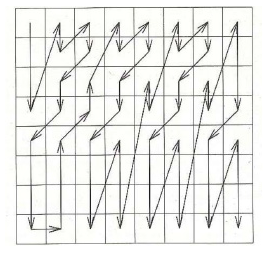
\includegraphics[width=10cm,height=10cm,keepaspectratio]{figuras/zigzag.png}
\end{center}
\caption{Método del zig-zag\cite{b1:2015}}
\label{fig_zigzag}
\end{figure}

El procesamiento de un GOP no es secuencial, al existir relaciones bidireccionales entre cierto tipo de frames. Al empezar un GOP, en primer lugar se procesa el I-frame. El siguiente frame a procesar será de tipo P, puesto que solamente necesita de este I-frame. Una vez procesados estos dos frames, los B-frames que están en medio serán decodificados. El proceso sigue alternando el procesamiento de P-frames con B-frames intermedios, hasta finalizar el GOP en cuestión, como se puede ver en \ref{fig_gop}.

\begin{figure}[ht!]
\begin{center}
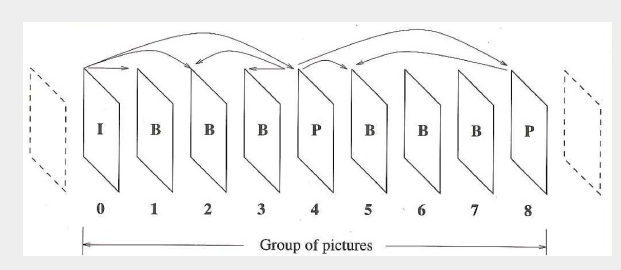
\includegraphics[width=10cm,height=10cm,keepaspectratio]{figuras/gop.png}
\end{center}
\caption{Procesamiento en GOP}
\label{fig_gop}
\end{figure}

\section{Procesamiento en sensores de imágenes} 
Existen principalmente dos tipos de sensores que se usan para capturar imágenes o vídeo: sensores CCD (del inglés \textit{Charge Coupled Device}) y sensores CMOS (del inglés \textit{Complementary Metal Oxide Semiconductor}). Ambos sensores se basan en el mismo principio que es capturar la máxima cantidad de luz que incide en el sensor y convertirla en una se\~al eléctrica que será transformada posteriormente en digital. Los sensores CMOS tratan los píxeles de forma individaul mientras que los sensores CCD se basan en la propagación de carga eléctrica mediante condensadores. En la actualidad, los sensores CMOS son ampliamente utilizados, sobre todo en dispositivos móviles, ya que los sensores CCD necesitan un chip adicional y son más costosos y grandes que los CMOS, por lo que en lo que sigue se detallará el funcionamiento de los sensores CMOS\cite{villalba:2015}. 

Un sensor CMOS consiste en una matrix de sensores de pixels, cada uno de ellos compuesto de un fotodetector y un amplificador activo. Cada uno de estos sensores de pixels captura información de un píxel en uno de los tres colores primarios (rojo, verde y azul) puesto que se aplica un filtro de color conocido como CFA (\textit{Color Filter Array}). Bayer es el CFA más utilizado, compuesto por un patrón de filtro que es la mitad verde, un cuarto azul y un cuarto rojo, debido a que el ojo humano es más sensible al color verde\ref{fig_cfa}\cite{b3:2012}. \\ 

\begin{figure}[ht!]
\begin{center}
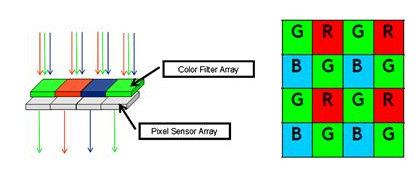
\includegraphics[width=10cm,height=10cm,keepaspectratio]{figuras/cfa.png}
\end{center}
\caption{Bayern CFA, \cite{b3:2012}}
\label{fig_cfa}
\end{figure}

Tras la aplicación del filtro CFA para cada píxel se tiene únicamente información sobre un color, lo que implica que se tiene que llevar a cabo un proceso para estimar los valores de los otros dos componentes del color. Esta estimación se puede realizar mediante distintas técnicas, todas ellas basadas en utilizar los valores de los píxels cercanos. Se pueden usar métodos sencillos como el del vecino más próximo (el píxel toma el valor del píxel que le precede) o el bilinear (toma como valor la media de sus vecinos en vertical y horizontal más próximos) u otros más complejos como pueden ser splines cúbicas, método de mínimos cuadrados o filtros direccionales\cite{b2:2005}.

Tras la conversión Bayer-RGB hay varias funciones que en función del dispositivo y sensor pueden aplicarse como pueden ser corrección del color o corrección gamma. \\

Hay que tener en cuenta que en este proceso el hardware tiene una influencia considerable. Cada sensor a pesar de pertenecer al mismo fabricante tiene peque\~nas imperfecciones o diferencias del resto que impactan directamente en la imagen obtenida. Esto es conocido como el ruido del sensor, que se aborda en la siguiente sección.

\section{Extracción del ruido en imágenes}
Los principales componentes del ruido en imágenes por imperfecciones del sensor son el FPN (\textit{Fixed Pattern Noise}) y el PRNU (\textit{Photo Response Non Uniformity}).

El ruido FPN se genera por la corriente oscura y depende también de la exposición y de la temperatura. Es un ruido independiente de las imperfecciones del sensor y es un ruido aditivo que es eliminado en algunas cámaras restando una capa de color negro.

El ruido PRNU es el mayoritario y es un ruido multiplicativo, lo que complica su eliminación. Está compuesto por dos ruidos: PNU (\textit{Pixel Non-Uniformity}) y por defectos de baja frecuencia como pueden ser la configuración del zoom, y la refracción de la luz en las lentes. Es el primero de estos dos componentes, el PNU, el que tiene que ver con la fabricación de los wafers de silicio y las imperfecciones en el proceso de fabricación, lo que hace que sea un atributo único de cada sensor. \\

La extracción del PRNU se basa en aplicar una función a la imagen original que elimine el ruido de la imagen, obteniendo la imagen limpia de ruido. Al substraer la imagen original de la imagen sin ruido obtenemos el ruido. En \cite{dabov:2007} usan el algoritmo BM3D y en \cite{gisolf:2013} proponen usar el algoritmo FSTV, en \cite{goljan:2006} usan transformadas de ondículas o \textit{wavelets} para eliminar el ruido. Este ruido puede estar contaminado por agentes externos, en consecuencia se han desarrollado técnicas como \textit{zero-mean}\cite{goljan:2008} o el filtro de Wiener\cite{wiki:wiener}.


\chapter{Análisis forense en vídeos digitales}
\pagestyle{fancy}
%\pagenumbering{arabic}
En este capítulo se presentan las principales técnicas forenses aplicadas a vídeos. A pesar de ser un campo ampliamente investigado, la gran cantidad de vídeo que se produce a diario y el crecimiento de aplicaciones de edición de vídeo para usuarios no expertos ha crecido exponencialmente en los últimos a\~nos, lo que hace que muchos de los algoritmos desarrollados queden desactualizados frente a nuevos técnicas antiforenses. 
La gran digitilización de la sociedad en los últimas décadas ha influido notablemente en procesos judiciales, especialmente posteriormente a $1978$ puesto que tras la legislación deFlorida se admitían pruebas digitales (e-mails, fotografías o vídeos digitales, audios, etc.) como evidencia. Para garantizar que pruebas digitales puedan considerarse como evidencia de sucesos reales tiene que garantizarse que no haya sido manipulada y debe poder establecerse la fuente de adquisión de los datos digitales en cuestión. \\

En las siguientes secciones se describen en detalle la detección de manipulación de vídeos, la detección de doble compresión (un caso concreto que permite la detección de manipulación de vídeos) y la identificación de la fuente.

\section{Manipulación de vídeos}
Actualmente existen multitud de herramientas de edición de vídeo a disposición de usuarios no expertos, que pueden manipular la imagen de múltiples formas como introduciendo, quitando, repitiendo o copiando frames, además de operaciones que no a\~naden objetos al vídeo como son la rotación, el escalado o la aplicación de filtros. En cualquiera de los dos casos, a pesar de que no haya a\~nadido o eliminado ningún objeto en frames, afectará a la codificación del vídeo. \\

La aplicación de técnicas forenses para imágenes para la detección de manipulaciones en vídeos no es recomendable. La estructura de los vídeos y los distintos tipos de frames del GOP permiten técnicas basadas en la consistencia temporal incapaces de ser detectadas por medio de análisis estáticos de los frames considerados como imágenes, además de ser algoritmos computacionalmente costosos y de ser incapaces de detectar la inserción o eliminación de frames\cite{bestagini:2012}. \\

En \cite{chang:2013} analizan el problema de la duplicación de frames y utilizan la correlación como medida de similitud. En primer lugar eligen un conjunto de segmentos candidatos de entre todos los del vídeo, reduciendo el espacio de búsqueda, para luego calcular la medida de similitud entre ellos a partir de histogramas de color y decidir si se ha producido duplicación o no. Para los experimentos han utilizado un conjunto de 15 vídeos manipulados y el algoritmo ha mostrado una precisión media del $85\%$. \\

En \cite{wu:2014} se centran en la detección de eliminación o duplicación de frames consecutivos. Para ello se basan en un término derivado de la velocidad de partículas en imágenes o PIV (del inglés \textit{Particle Image Velocity}), cuya idea es comparar frames adyacentes y estimar el desplazamiento causados por la separación en el tiempo. La duplicación o eliminación de frames consecutivos contribuye a aumentar este desplazamiento. Para decidir si un desplazamiento concreto es debido a una manipulación, utilizan el test de Grubbs\cite{wiki:grubbs} que para una distribución normal permite detectar \textit{outliers}. En los experimentos parten de $40$ vídeos a partir de los que generan otros $40$ eliminando frames y otros $40$ duplicando frames. La precisión media es del $96,3\%$ con una tasa de falsos positivos del $10\%$. \\

En \cite{wang:2014} se basan en que la correlación entre los coeficientes de valores grises es consistente en vídeos pero cuando se produce una falsificación desaparece esta consistencia. Primero extraen la consistencia de la correlación de los coeficientes de los valores grises para posteriormente clasificar las características mediante SVM (del inglés \textit{Support Vector Machine}). En los experimentos parten de una base de datos de vídeos originales y crean otras cuatro bases de datos a partir de los originales con las siguientes manipulaciones: insertando $25$ frames, insertando $100$ frames, eliminando $25$ frames y eliminando $100$ frames. Para entrenar la SVM utilizan $480$ vídeos originales y $480$ vídeos falsificados, dejando $118$ originales y otros tantos manipulados para pruebas, consiguiendo precisiones por encima del $90\%$. \\

Los mismos autores, en \cite{flow:2014} utilizan otro método basado también en la consistencia temporal entre frames. En este caso en lugar de utilizar la correlación entre los coeficientes grises, utilizan la consistencia medida mediante el flujo óptico de Lucas-Kanade que permite determinar el movimiento de un objeto dentro de una secuencia de frames. Para los experimentos utilizan la mismas bases de datos que en el caso anterior y una SVM para la clasificación, consiguiendo una precisión media superior también al $90\%$. \\

En \cite{kingra:2017} se basan en el flujo óptico pero lo calculan siguiendo Horn-Schunck en lugar de Lucas-Kanade. Extraen únicamente los frames tipo I y tipo P y extraen como características el PRG (del inglés \textit{Prediction Residual Gradient}) y el OFG (del inglés \textit{Optical Flow Gradient}), el primero centrado en variaciones en la posición de objetos mientras que el segundo está centrado en cambios en la luminosidad. Estas dos características son comparadas con unos umbrales determinados empíricamente para detectar picos, cuando los picos sean continuos se tratará de una manipulación. El método ha mostrado una precisión de un $86\%$ en las pruebas realizadas. \\

En \cite{jia:2018} utilizan también el flujo óptico de Lucas-Kanade para detectar inconsistencias en el caso de manipulaciones de tipo inserción o eliminación de frames. En lugar de computar la correlación entre frames del flujo óptico primero utilizan un estadístico que resume la información de los vectores resultantes de Lucas-Kanade para comprobar la consistencia con estos. Cuando se detectan irregularidades en base a este estadístico calculan la correlación entre los vectores completos del flujo Lucas-Kanade. Utilizan para las pruebas un total de $115$ vídeos con una precisión en torno al $90\%$. \\

Algunos autores han desarrollado métodos basados en la extracción de algún tipo de huella a partir de los frames que componen el vídeo para detectar anomalías en frames con huellas significativamente distintas. Estos métodos tienen el incoveniente de que los vídeos comprimidos pierden mucha información sobre la huella, y solamente han demostrado dar buenos resultados en vídeos no comprimidos que suele ser poco usual. En \cite{mondaini:2007} obtienen el PRNU de los primeros frames que componen el vídeo y utilizan distintas medidas para detectar ataques como inserción de \textit{frames}, inserción de objetos y replicación de frames mediante la correlación entre el PRNU de referencia del vídeo y el ruido de un frame en concreto, la relación entre el ruido de dos frames consecutivos o la relación entre dos frames consecutivos. En \cite{kobayashi:2010} utilizan en lugar del PRNU un ruido que solamente es aplicable a los sensores CCD, el ruido del fotón en disparo. Además, su método solamente es aplicable a vídeos grabados de forma estática sin la cámara en movimiento lo cual restrige mucho el ámbito de aplicabilidad del algoritmo. En el caso en el que se den las premisas de las que parten el método tiene una precisión del $97\%$. \\

Aprovechando la consistencia entre frames de tipo temporal, algunas investigaciones se han centrado en aspectos de tipo geométrico como pueden ser que las propiedades físicas o de iluminación sean reales. En \cite{conotter:2011} se utilizan técnicas geométricas para detectar trayectorias imposibles de objetos en vuelo libre. Para ello, se modeliza el movimiento parabólico de estos objetos en tres dimensiones para proyectar este modelo posteriormente en dos dimensiones y compararlo con la trayectoria de ese mismo objeto en el vídeo. El método desarrollado es válido tanto para cámaras estáticas como para cámaras en movimiento y se han realizado experimentos con diversos vídeos ya sea generados por ellos u obtenidos de plataformas de compartición de contenido en los que han medido el error medio entre la trayectoria real y la trayectoria estimada mediante su procedimiento para ser capaces de clasificar cuando una trayectoria ha sido falseada, sin embargo no han datos sobre la precisión del algoritmo en cuestión. Hay que tener en cuenta que esta técnica solamente puede ser utilizada en vídeos en los que exista un objeto que describa una trayectoria parabólica y por tanto no es válida para cualquier vídeo. \\

Sin embargo, la mayoría de trabajos sobre la detección de manipulación de vídeos están basados en detectar la re-comprensión o doble compresión de un vídeo, puesto que al ser editado se vuelve a comprimir por segunda vez. 

\section{Doble compresión}
Gran parte de los estudios sobre doble compresión se centran en vídeos con formato MPEG y utilizan las mismas ideas que en la detección de doble compresión de imágenes JPEG. En concreto, la re-cuantificación afecta de los coeficientes con un paso de cuantificación distinto del original afecta al histograma de los coeficientes DCT\cite{bestagini:2012}. Estos coeficientes pueden ser aproximados como\cite{fridrich:1998}

\begin{equation}
Y_{Q_1, Q_2} = \Delta_{2} sign(Y)round\left(\frac{\Delta_1}{\Delta_2}round\left(\frac{|Y|}{\Delta_1}\right)\right) \nonumber
\end{equation}

siendo $\Delta_1$ y $\Delta_2$ el tama\~no del paso en la primera y segunda compresión, respectivamente.

En \cite{fridrich:2003} muestran como la relación que hay entre $\Delta_1$ y $\Delta_2$ influye en el histograma creando un máximo característico. Intuitivamente, la idea es que al descomprimirse la imagen, modificarse una porción de la misma y volverse a comprimir, esa porción modificada mostrará trazas de una sola compresión mientras que el resto de la imagen tendrá rasgos de doble compresión. 

En \cite{huang:2014} presentan un método para el caso en el que se ha utilizado la misma matriz de cuantificación en ambas compresiones, basado  en el número de coeficientes DCT distintos que hay en una compresión, doble compresión y triple compresión.

En \cite{wang:2013} utilizan un conjunto de clasificadores binarios entrenados con distintas combinaciones entre $\Delta_2$ que es conocida (se puede leer directamente de los datos del vídeo) y posibles $\Delta_1$, para luego tomar el voto de la mayoría con las características concretas del vídeo en cuestión. \\

En \cite{tariang:2017} se basan en aplicar que se obtiene lo mismo si se comprime la imagen una vez con $\Delta_1$ que si se comprime dos veces con la misma matriz de cuantificación $\Delta_1$. De esta forma, dada la imagen original vuelven a comprimirla con distintas matrices hasta encontrar una que cumpla que en la mayoría de los bloques codificados se htenga la imagen original, obteniendo así la matriz de cuantificación que se utilizó en la última compresión. La manipulación se detecta en el caso de que existan algunos bloques distintos en la imagen comprimida que en la original puesto que entonces la última compresión no ha sido aplicada por igual en todos los bloques y ha existido una doble compresión. Para la experimentación contaron con un conjunto de $1338$ imágenes y dentro de las pruebas que realizaron la peor precisión media que obtuvieron fue del $88,7\%$. Es importante tener en cuenta que si la imagen ha sido manipulada y se ha utilizado la misma matriz de cuantificación que en la primera compresión, este método no logrará detectarlo. \\

En \cite{sun:2013} se extraen los coeficientes DCT para luego calcular las diferencias entre ellos en cuatro direcciones: horizontal, vertical, diagonal mayor y diagonal menor. Tras obtener estas cuatro matrices se truncan algunos elementos basados en ciertos umbrales para luego ser modeladas cada uno por medio de un proceso aleatorio de Markov de primer orden. Tras algunas transformaciones sobre estos procesos de Markov, se crea un array de características que será tratado por algoritmos de \textit{machine learning} puesto que la doble compresión conlleva unos errores de redondeo que dejan muestras estadísticas caracterizables por Markov. Para la experimentación generan $5040$ vídeos con la misma estructura GOP y con distintas combinaciones $\Delta_1$ y $\Delta_2$, con una precisión superior al $90\%$. \\

Otra estrategia ampliamente utilizada se basa en que mientras que los coeficientes DCT de una imagen siguen una distribución Laplace\cite{reininger:1983} o una distribución Cauchy\cite{eggerton:1986}, también siguen la ley de Benford\cite{fu:2009}, esto es, el primer dígito significativo es $d$ con probabilidad $\log_{10}\left(1+\frac{1}{d}\right)$. Si los coeficientes DCT se alejan significativamente de esta distribución entonces podemos concluir que se ha utilizado doble compresión. Muchas investigaciones han utilizado procedimientos basados en la ley de Benford aplicados al caso de doble compresión JPEG en imágenes, extensibles al caso de vídeo. 

En \cite{wang:2009} parten de la hipótesis que el factor de multiplicación $q_1$ de la tabla de cuantificación y el factor $q_2$ de la segunda tabla de cuantificación varían mientras que la tabla se mantiene la misma. En el caso de que $q_1 > q_2$ se observan anomalías en el histograma de los coeficientes DCT de tipo AC (frecuencia distinta de cero en ambas dimensiones espaciales) distintos de cero y es posible detectar la doble compresión. \\

En \cite{milani:2012} aplican la ley de Benford para un subconjunto de las frecuencias del DCT que identifican más sensible al número de compresiones y utilizan un multiclasificador compuesto de $N$ clasificadores SVM $S_k (k=1, \dots, N)$ donde $S_k$ es un clasificador binario que detecta si la imagen ha sido comprimida $k$ veces o no. De esta forma el número de compresiones que ha sufrido la imagen se toma como el clasificador con mayor $k$ que haya detectado que ha sido comprimido $k$ veces. Para la experimentación se ha trabajado con un conjunto de prueba de $100$ imágenes y un conjunto de test de $10$ imágenes, donde han obtenido una precisión del $94\%$ considerando que como máximo podía haber $N=4$ compresiones.

En \cite{chen:2009} aplican la ley de Benford para vídeos puesto que la codificación MPEG para vídeos y JPEG para imágenes comparten el mismo proceso. Observan que cuando se utiliza VBR los coeficientes AC distintos de cero de los I-frames doblemente comprimidos se alejan de la ley de Benford solamente cuando la escala de cuantificación utilizada en $\Delta_2$ es menor que la utilizada en $\Delta_1$. En el caso de CBR sí que aprecian compartamientos anómalos sin distinción de casuística. Para formalizar lo anterior, utilizan clasificadores binarios SVM en los que tratan como unidad un GOP decidiendo que existe doble compresión si el porcentaje de frames detectados como doblemente comprimidos excede un umbral determinado, obteniendo una precisión media superior al $95\%$. \\

Los métodos descritos arriba se basan en extender técnicas desarrolladas para imágenes para el caso de vídeo. Sin embargo, existen otros algoritmos que aprovechan la alteración de la estructura GOP de los vídeos. Dentro de un GOP, los P-frames están correlacionados con el I-frame inicial, de forma que en caso de existir doble compresión los frames que cambien de GOP, ver figura \ref{fig_doble-compresion} mostrarán ciertas características estadísticas.

En \cite{farid:2009} se centran en el error de movimiento o compensación de movimiento de los P-frames, esto es, la transformación que se debe aplicar a un frame de tipo I o de tipo P anterior para obtener el P-frame en cuestión. Al deshacerse la secuencia original GOP, existirán P-frames cuyo frame de referencia haya cambiado y el error de movimiento en ese caso es mayor. En este trabajo no se describe el método para determinar el umbral que determine si el error de movimiento corresponde con un cambio en la estructura GOP ni tampoco se dan resultados concretos sobre la precisión del algoritmo. 

En \cite{yao:2017} analizan las características periódicas del \textit{string} de bits de datos y del \textit{skip macroblocks} para todos los I-frames y P-frames. Los \textit{skip mabroblocks} son usados en P-frames y B-frames y no contienen información, correspondientes a macrobloques en los que no se producen cambios respecto del I-frame sobre el que se codifican. Muestran como al cambiar la estructura GOP el número de \textit{skip macroblocks} decrece puesto que el I-frame original en el que se basaba el P-frame era antes un P-frame.

En \cite{vazquez:2012} utilizan el número de \textit{inter-coded macroblocks} y de \textit{skip macroblocks} de cada frame modelizados como $i(n)$ y $s(n)$, cuando se produce un pico en $s(n)$ hay una alta probabilidad de doble compresión y el I-frame del que toma los valores fuera anteriormente un frame de tipo P, utilizando un razonamiento análogo al caso anterior. \\

\begin{figure}[ht!]
\begin{center}
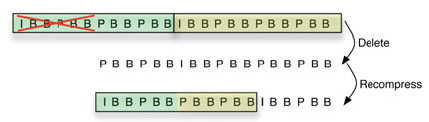
\includegraphics[width=10cm,height=10cm,keepaspectratio]{figuras/doble-compresion.png}
\end{center}
\caption{Reestructuración de GOP tras doble compresión, \cite{bestagini:2012}}
\label{fig_doble-compresion}
\end{figure}

\section{Identificación de la fuente}
La identificación de la fuente de adquisición es de vital importancia para muchos procesos judiciales, podría compararse con las pruebas balísticas para identificar un arma. Es por esto por lo que la identificación de la fuente en imágenes ha sido ampliamente estudiado por académicos en los últimos a\~nos con buenos resultados. 
Esta sección se restringe a la identificación de la fuente entendido como la identificación del modelo fuente en dispositivos móviles y no engloba otras temáticas como podría ser distinguir entre gráficos generados por ordenador o capturados. 

Existen muchas menos investigaciones sobre esta materia en vídeo que en lo referente a imagen, a pesar de que un vídeo se descompone como una secuencia de frames. Sin embargo, la menor resolución en vídeo frente a imagen y las altas compresiones que se utilizan hacen que se pierde mucha información sobre la huella. \\

En \cite{naveen:2016} extran una serie de fotogramas del vídeo en base a la luminosidad para extraer el PRNU mediante la descomposición \textit{wavelet} de Daubechies de cuarto nivel a los que se aplica el filtro de Wiener. Se computa la correlación entre el ruido de cada frame para posteriormente evaluarlo mediante PCE (del inglés \textit{Peak-to-Correlation Energy}). Se utiliza un método de clasificación en el que las imágenes a analizar son caracterizadas en uno u otro grupo según el PCE. \\

En \cite{chen:2007} tratan el vídeo como una secuencia de $N$ frames, para cada uno de esos frames extraen el PRNU y utilizan el estimador de máxima verosimilitud para identificar el PRNU del vídeo. Para decidir si dos vídeos fueron tomados por la misma cámara se basan en la covarianza normalizada y en el PCE: si provienen del mismo dispositivo entonces el PCE es grande por el pico en la covarianza normalizada y en caso de no provenir de la misma fuente la covarianza normalizada parecerá ruido blanco. En las pruebas se utilizaron $25$ cámaras y muestra como el nivel de compresión del vídeo es crucial para el algoritmo, cuanta mayor compresión menor calidad y más tiempo de vídeo (en algunos casos $10$ minutos de vídeo) se necesita para obtener un PRNU suficientemente bueno, lo que hace que este método no sea efectivo para vídeos de corta duración grabados por móvil. \\ 

En \cite{yahaya:2012} utilizan un subconjunto de los coeficientes AC de la transformada DCT formado a partir de tres índices $p$, $q$ y $r$ que toman $8$ orientaciones diferentes. Para cada una de esas orientaciones se calculan $9$ estadísticos en base a la relación de orden entre $p$ y $q$ y entre $r$ y $q$ lo que da un total de $72$ estadísticos diferentes que denominan caracerísticas CP, también utilizados en otros trabajos de estegoanálisis, que utilizarán como \textit{input} para un clasificador de tipo SVM. Para las pruebas utilizan $4$ modelos de cámara diferentes y $10$ vídeos de cada una de ellas, obteniendo una precisión del $100\%$. \\

En \cite{dong:2010} utilizan características propias de la codificación MPEG-2, características relacionadas con la tasa de bits, los factores de cuantificación y los vectores de movimiento. Tanto la tasa de bits como los factores de cuantificación y los vectores de movimiento no son parámetros fijos en el estándar MPEG-2, cada fabricante establece unos en concreto según el sensor. Tras extraer estas características, se utiliza un clasificador SVM entrenado. Para las pruebas utilizan vídeos de ocho diferente codificadores y obtienen precsiones por encima del $86\%$. Hay que tener en cuenta que vídeos obtenidos de cámaras que compartan el mismo codificador de MPEG-2 no serán clasificados como distintos por lo que este método solamente sirve para garantizar que dos vídeos provienen de distinta fuente. \\

En \cite{gprnu:2016} se basan en que dentro de los canales RGB el verde es el que tiene más información sobre la huella. Por ello extran el canal verde de la imagen y mediante interpolación bilineal redimensionan los frames a tama\~no $512$x$512$ a los que extraen el ruido mediante \textit{soft-thresholding}. El PRNU del vídeo lo obtienen como la media de los ruidos de cada frame y los clasifican utilizando la correlación como medida de similitud. En las pruebas muestra cómo los resultados de este proceso con el G-PRNU (\textit{Green PRNU}) son mejores que con el PRNU. \\


\chapter{Clustering}
\pagestyle{fancy}
%\pagenumbering{arabic}
En este capítulo se describe el clustering y dos métodos principales. También se comentan varios métodos para elegir el número óptimo de clusters. \\

Clustering es una técnica de aprendizaje no supervisado que a partir de un conjunto de datos y una medida de similitud o distancia entre ellos los agrupa en distintas clases o clusters de forma que elementos que están en el mismo clúster son más parecidos entre ellos que con los de otro clúster distinto. \\

En primer lugar se describen los algoritmos de clustering más utilizados y posteriormente se comentarán métodos para elegir el número de clases o clusters óptimo. \\

\section{K-means}
El algoritmo de clustering K-means agrupa $n$ elementos en $k$ clusters $S_k$ con el objetivo de minimizar la suma del error cuadrático intra-cluster:

\begin{equation}
\sum_{i=1}^{k}\sum_{x\in S_i}\lVert x-\mu_{i}\rVert ^2 \nonumber
\end{equation}

donde $\mu_i$ es la media de las distancias entre los elementos en $S_i$, también conocidos como centroides. \\

La suma del error cuadrático intra-cluster o inercia es un indicador de la cohesión de los clusters. A mayor cohesión, menor distancia existirá entre los elementos de cada clúster y por tanto también del centroide. Este indicador sin embargo tiene ciertas desventajas:
\begin{itemize}
\item Asume que los clusters se modelan como esferas, al estar basado en $k$ centroides y minimizar la distancia euclídea, lo que implica misma varianza entre clusters. Ver \ref{fig_kmeans1}.
\item No es una métrica normalizada
\item Muy sensible a outliers al utilizar la distancia al cuadrado
\item No tiene en cuenta la densidad de cada cluster. Implícitamente asume que al ocupar cada clúster el mismo área cada cluster tiene que tener el mismo número de puntos. Ver \ref{fig_kmeans2}.
\end{itemize}

\begin{figure}[ht!]
\begin{center}
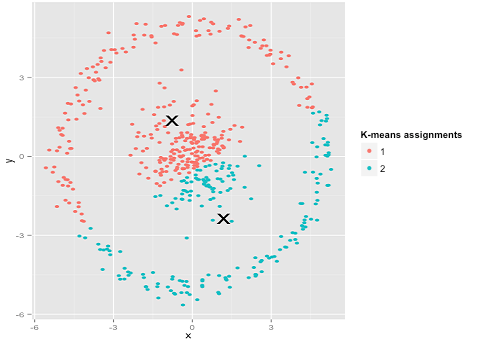
\includegraphics{figuras/kmeans1.png}
\end{center}
\caption{K-means frente a varianza en clusters}
\label{fig_muestreo}
\end{figure}

\begin{figure}[ht!]
\begin{center}
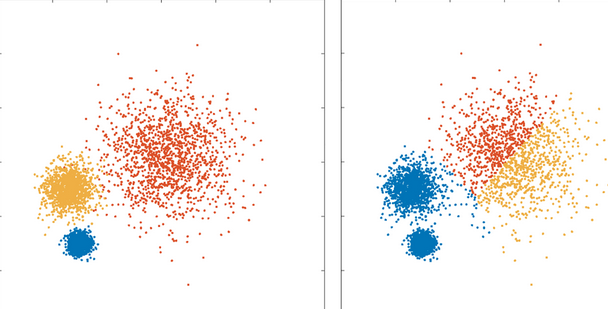
\includegraphics[width=10cm,height=10cm,keepaspectratio]{figuras/kmeans2.png}
\end{center}
\caption{K-means no es sensible a la densidad de puntos}
\label{fig_kmeans2}
\end{figure}

Dado un conjunto de $n$ elementos $\{x_1, x_2, \dots, x_n\}$ K-means empieza con una fase de inicialización en la que se escogen $k$ centroides, $\{c_1, c_2, \dots, c_k\}$. Una vez elegidos los centroides, itera de la siguiente forma: 
\begin{itemize}
\item \textbf{Etapa de asignación}: asigna cada elemento al centroide que minimiza la distancia euclídea al cuadrado, el cluster $S_i$ que tiene como centroide $c_i$ es
\begin{equation}
S_i = \{x_j : \lVert x_j - c_i \rVert ^2 \leq \lVert x_j - c_p \rVert ^2 \; \forall p, 1\leq p \leq k\} \nonumber
\end{equation}
\item \textbf{Actualización de los centroides}: serán la media de los elementos del cluster correspondiente.
\begin{equation}
c_i = \frac{1}{\displaystyle |S_i|}\sum_{x_j \in S_i}x_j \nonumber
\end{equation}
\end{itemize}

Cuando en la etapa de asignación no se producen cambios entre dos iteraciones consecutivas, el algoritmo termina. \\

La inicialización de los centroides es un aspecto muy relevante en el algoritmo: K-means converge cuando encuentra un óptimo local por lo que se han desarrollado diversos métodos de inicialización de forma que se encuentre el óptimo global:
\begin{itemize}
\item Aleatorio: se asigna de forma aleatoria un elemento a cada cluster y posteriormente se calculan los centroides en base a esta asignación. Este método ubica los centroides cerca del centro del conjunto de datos.
\item Forgy: se escogen al azar $k$ elementos del conjunto y se utilizan como centroides. Este método tiende a dispersar los centroides iniciales.
\item MacQueen: escoger al azar $k$ elementos del conjunto y tratarlos como centroides. Asigna cada elemento al cluster con el centroide más próximo y recalcula los centroides, que serán los centroides de inicialización para el algoritmo.
\item K-means++: propuesto en el a\~no 2007. Funciona de la siguiente forma:
    \begin{enumerate}
    \item Se elige un centroide elegido aleatoriamente sobre el conjunto de observaciones.
    \item Se calcula la distancia al cuadrado entre cada observación y el centroide seleccionado.
    \item Se elige otro punto al azar como segundo centroide, la probabilidad que tiene cada observación de ser elegido es proporcional a la distancia al cuadrado calculada en (2).
    \item Repetir (2) y (3) hasta tener $k$ centroides.
    \end{enumerate}
\end{itemize}

En los últimos a\~nos se ha utilizado ampliamente la inicialización mediante K-means++, además de ejecutar varias veces el algoritmo con distintos centroides para evitar óptimos locales. \\

\section{Clustering jerárquico}
El clustering jerárquico se refiere a una familia de algoritmos de clustering que construyen clusters de forma anidada al fusionarlos (clustering aglomerativo) o dividirlos (clustering divisivos). 

Cuando se trata de clustering aglomerativo, dado un conjunto de $n$ elementos cada uno constituirá un cluster y en cada iteración se fusionarán dos clústers de forma que se minimize la medida de distancia o similitud especificada, terminando el algoritmo cuando haya $1$ cluster.

En el caso de clustering divisivo, dado un conjunto de $n$ observaciones se agrupan en un único cluster y se producen sucesivas divisiones, terminando cuando haya $n$ clusters. \\

En cualquiera de los dos casos, las sucesivas iteraciones son representadas a través de un dendrograma. Como se puede ver en \ref{fig_dendrograma} un dendrograma es un diagrama en forma de árbol. En este caso muestra un algoritmo de clustering aglomerativo en el que los elementos $\{a, b, c, d, e, f\}$ se han ido agrupando en sucesivas iteraciones hasta terminar con $1$ cluster. \\

\begin{figure}[ht!]
\begin{center}
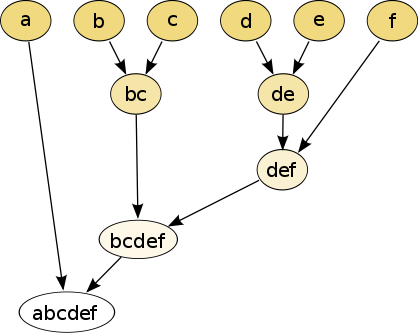
\includegraphics[width=10cm,height=10cm,keepaspectratio]{figuras/dendrograma.png}
\end{center}
\caption{Dendrograma\cite{wiki:dendrogram}}
\label{fig_dendrograma}
\end{figure}

En lo sucesivo se contemplará el clustering aglomerativo, los conceptos y métodos para el caso divisivo son análogos. Para decidir cómo agrupar los clusters de forma iterativa es necesario definir una medida de similitud entre clusters, de forma que clusters similares se agrupen antes que clusters distintos. En la primera iteración en la que todos los clusters están compuestos por un único elemento se puede especificar una distancia, en el resto de iteraciones será necesario definir un criterio de enlace o \textit{linkage criteria} que modele cómo medir la similitud entre dos clusters en los que al menos uno de ellos está compuesto por más de una observación. \\

Se puede especificar cualquier distancia $d$, mientras cumpla las propiedades de distancia desde un punto de vista matemático, que son:
\begin{itemize}
\item $d(x,y) \geq 0$ y $d(x,y)=0 \iff x=y$
\item $d(x,y) = d(y,x)$ o propiedad simétrica
\item $d(x,z) \leq d(x,y) + d(y,z)$ o desigualdad triangular
\end{itemize}

Las distancias más habituales son las siguientes:
\begin{itemize}
\item Distancia euclídea. La más común y la que se utiliza por defecto.
    \begin{equation}
    d(x,y) = \sqrt{\sum(x_i-y_i)^2} \nonumber
    \end{equation}
\item Distancia del taxi, también conocida como distancia Manhattan debido al dise\~no en cuadrícula de las calles de la isla.
    \begin{equation}
    d(x,y) = \sum |x_i - y_i| \nonumber
    \end{equation}
\item Distancia de Chebyshev, también conocida como distancia del tablero de ajedrez ya que coincide con el número de movimientos que necesita el rey para moverse de una casilla a otra.
    \begin{equation}
    d(x,y) = \max{|x_i - y_i|} \nonumber
    \end{equation}
\item Distancia de Hamming, para vectores lógicos, es el número de bits que tienen que cambiarse para transformar un vector de bits en otro.
    \begin{equation}
    d(x,y) = \frac{\displaystyle c_{01} + c_{10}}{\displaystyle n} \nonumber
    \end{equation}
donde $c_{ij}$ es el número de ocurrencias de $x[k] = i, y[k] = j$ para $k < n$. 
\item Distancia de Mahalanobis. Distancia muy útil para determinar la similitud entre dos variables aleatorias multidimensionales al tener en cuenta la correlación y la escala de ellas.
    \begin{equation}
    d(x,y) = \sqrt{(x-y)V^{-1}(x-y)^T} \nonumber
    \end{equation}
donde $V$ es la covarianza y $V^{-1}$ la inversa de la matriz de covarianza.
\end{itemize}

Además, otras que son ampliamnete utilizadas son Bray-Curtis, Canberra, coseno, Minkowski, o la euclídea normalizada. Para el caso de variables booleanas, además de la ya mencionada arriba distancia Hamming se han empleado: dado, Jaccard-Needham, Kulsinski, Rogers-Tanimoto, Russell-Rao, Sokal-Michener, Sokal-Sneath y Yule. \\

Una vez definidas la distancia a utilizar entre cada par de observaciones, se pueden definir distintos criterios de enlace entre dos clústers $u$ y $v$. Los más habituales son los siguientes:
\begin{itemize}
\item Método \textit{single} o del punto más cercano. 
    \begin{equation}
    d(u,v) = \min{(dist(u[i], v[j]))} \nonumber
    \end{equation}
para todos los puntos $i$ en el cluster $u$ y todos los $j$ en $v$. Este algoritmo se centra en la separación entre clusters pero no en la cohesión de los clusters y permite formas geométricas más flexibles que en otros casos.
\item Método \textit{complete}, también conocido como Algoritmo del punto lejano o Algoritmo de Voor Hees.
    \begin{equation}
    d(u,v) = \max{(dist(u[i], v[j]))} \nonumber
    \end{equation}
\item Método \textit{average} o algoritmo UPGMA.
    \begin{equation}
    d(u,v) = \sum_{ij}\frac{\displaystyle dist(u[i], v[j])}{(|u| * |v|)} \nonumber
    \end{equation}
\item Método \textit{weighted} o algoritmo WPGMA,
    \begin{equation}
    d(u,v) = (dist(s,v) + dist(t,v))/2
    \end{equation}
donde el cluster $u$ está compuesto por los clusters $s$ y $t$.
\item Método \textit{centroid} asigna como distancia entre clusters la distancia euclídea entre sus centroides.
\item Método \textit{ward}. Según Ward la distancia entre dos clusters $u$ y $v$ es el incremento que se producirá en la suma del error cuadrático si se fusionan:
    \begin{equation}
    d(u,v) = \sqrt{\frac{|v|+|s|}{T}d(v,s)^2 + \frac{|v|+|t|}{T}d(v,t)^2 - \frac{|v|}{T}d(s,t)^2}
    \end{equation}
donde $u$ es el nuevo cluster creado a partir de $s$ y $t$ y $T=|v|+|s|+|t|$. En este caso, a diferencia de K-means, el número de puntos interviene en la fórmula por lo que dados dos pares de clusters cuyos centros están distanciados por igual, el algoritmo de Ward fusionará los de menor cardinalidad.
\end{itemize}

\section{Elección del número de clusters óptimo}
Los algoritmos de clustering se utilizan principalmente de dos propósitos distintos según la problemática:
\begin{itemize}
\item Se conoce a priori el número de distintas clases en la población y se quieren obtener los cortes en el vector de características de las observaciones para conocer qué características tiene cada clase. Nuevas observaciones podrán ser categorizadas a partir del conocimiento extraído en el clustering.
\item No se conoce cuántas clases distintas existen en la población y se quiere conocer esto a partir del clustering.
\end{itemize}

Es en el segundo caso en el que no se tiene información sobre el $k$ a utilizar en el algoritmo K-means o el corte a aplicar en el dendrograma en clustering jerárquico. En lo que sigue se describen distintos métodos basados en heurísticas para determinar el número de clusters óptimo. \\

\subsection{Coeficiente silueta}
Para cada observación $x$ se tienen dos medidas:
\begin{itemize}
\item Cohesión $a(x)$: grado de similitud del elemento respecto del cluster. Se obtiene como la distancia promedio de $x$ a todos los puntos en el mismo cluster. 
\item Separación $b(x)$: grado de disimilitud del elemento respecto a elementos que han sido identificados en otras clases. La separación más utilizada es la distancia promedio entre $x$ y todos los elementos del cluster más cercano, aunque también se utilizan otras medidas para valorar la separación.
\end{itemize}

El coeficiente silueta para $x$ se define entonces como
\begin{equation}
s(x) = \frac{\displaystyle b(x) - a(x)}{\displaystyle \max{\{a(x), b(x)\}}} \nonumber
\end{equation}

y para todo el agrupamiento es
\begin{equation}
SC = \frac{1}{n}\sum_{x}s(x)
\end{equation}

donde $n$ es el número de observaciones. \\

Intuitivamente, un agrupamiento bien definido debería corresponderse con que para cada elemento $x$ se tiene que $a(x) << b(x)$, es decir, $x$ está muy cercano respecto de los elementos de su cluster en comparación con los elementos del cluster más cercano. El coeficiente $s(x)$ toma los valores en el rango $\left[ -1, 1\right]$, donde $-1$ corresponde con una mala elección del número de clusters y $1$ indica clusters bien definidos. \\

De esta forma, una de las técnicas que se usa con el coeficiente silueta es elegir un rango de valores para $k$, y elegir $k$ de forma que el coeficiente silueta para el agrupamiento sea máximo.

\subsection{Índice Calinski-Harabasz}
Dado $k$, se define el índice de Calinski-Harabasz como:
\begin{equation}
s(k) = \frac{SS_B}{SS_W} * \frac{N-k}{k-1} \nonumber
\end{equation}
$SS_B$ es la varianza entre clusters
\begin{equation}
SS_B = \sum_{i=1}^{k}n_id(m_i, m)^2 \nonumber
\end{equation}
donde $m_i$ es el centroide del cluster $i$ y $m$ es la media de todas las observaciones.

$SS_W$ es la varianza intra-cluster:
\begin{equation}
SS_W = \sum_{i=1}^{k}\sum_{x\in S_i}d(x, m_i)^2 \nonumber
\end{equation}

Para que los clusters estén bien definidos deben tener valores grandes para $SS_B$ (medida de separación) y peque\~nos para $SS_W$ (medida de cohesión). De esta forma el índice de Calinski-Harabasz es una adaptación del método F-test de ANOVA, $SS_B$ con $k-1$ y $SS_W$ con $n-k$ grados de libertad por lo que aparecen en la fórmula pues $SS_B$ debe ser proporcional a $k-1$ y $SS_W$ proporcional a $n-k$.  \\

Al igual que el coeficiente silueta, es un método que funciona generalmente bien para clusters convexos.

\subsection{Método del codo}


\chapter{Contribución}
%\pagestyle{fancy}
%\pagenumbering{arabic}
En este capítulo se presenta la contribución propia, un método de identificación de la fuente de adquisión de vídeos de dispositivos móviles en escenarios abiertos.

\section{Consideraciones generales}
El algoritmo desarrollado se puede divir en etapas. \\

En primer lugar se extraen los fotogrames de tipo I del vídeo puesto que contienen más información que el resto y de estos se selecciona un subconjunto de ellos en base a la similitud entre ellos, de forma que los fotogramas extraídos representen sin sesgo las diferentes escenas del vídeo, para evitar que frames con la misma escena contaminen el ruido. Para esto último se utiliza el algoritmo \textit{phash} que mide el grado de similitud entre distintos frames. \\

Una vez se han obtenido los fotogramas clave se extrae el PRNU de cada fotograma mediante el algoritmo desarrollado en \cite{ana:2015} basado en la transformada \textit{wavelet} de Daubechies y se define el sensor de la cámara como la media del ruido extraído de los frames clave. \\

El último paso corresponde con clustering jerárquico utilizando el método Ward puesto que se ha visto en las pruebas que es el que mejor resultado otorga en este contexto. De la misma forma, se ha validado experimentalmente que el método del codo es el que determina con mayor precisión el número de clusters óptimos. \\

\section{Especificación del método}
En el diagrama de cajas\ref{fig_metodo} se resume el algortimo propuesto, que consta de las siguientes fases:
\begin{enumerate}
\item Toma como entrada un conjunto de $n$ vídeos correspondientes a $m$ cámaras de móvil distintas.
\item \textbf{Extracción de fotogramas de tipo I}: mediante la herramienta \textit{ffprobe} se decodifica cada vídeo y se extraen los I-frames, que al haber sido comprimidos sin referenciar otros fotogramas contienen mayor grado de información que los P-frames o B-frames. Como se muestra mediante experimentos, el alto nivel de compresión de los fotogramas de tipo P y de tipo B evitan la obtención de una huella significativa a partir de estos por lo que es necesario buscar los fotogramas con menor nivel de compresión en vídeo que son los de tipo I. Aún así, la compresión de los I-frames es bastante alta en comparación a imágenes.
\item \textbf{Extracción de fotogramas clave}: para no contarminar el ruido con la escena, se deben elegir frames que representen las distintas escenas del vídeo. Para ello en primer lugar se computa el \textit{phash} de cada frame y se construye la matriz de distancias $D(i,j)$ para cada par de frames, utilizando la distancia Hamming. Para seleccionar los más disimilares se define un umbral determinado y el primer I-frame como fotograma clave. Se elijen los demás I-frames de forma que la distancia Hamming entre todos ellos sea mayor al umbral.
\item \textbf{Extracción del PRNU}: se extrae el PRNU de cada fotograma clave y se calcula el PRNU del vídeo como la media de los PRNU de los frames clave. 
\item \textbf{Matriz de distancias para clustering jerárquico}: se computa la correlación entre ruidos y se utiliza como matriz de distancias en un algoritmo de clustering jerárquico aglomerativo. Al tratarse de un escenario abierto, no se tiene una base de datos que asocia sensores a ruido PRNU por lo que es necesario agrupar los vídeos de entrada en grupos de forma que cada grupo represente un dispostivo distinto. 
\item \textbf{Elección del número de clusters óptimo}: el número óptimo de clusters se obtiene mediante el método del codo.
\end{enumerate}

A continuación se detalla el algoritmo de extracción de fotogramas clave.

\begin{algorithm}
\caption{Extracción de fotogramas clave}
\label{alg_keyframes}
\begin{algorithmic}[1]
\Statex \textbf{Input} video, secuencia de fotogramas
\Statex \textbf{Output} fotogramas clave
\State $iframes \gets extraerIframes(video)$
\State $hashes \gets phash(iframes)$
\State $dist \gets matrizDistancias(hashes)$
\State $umbral \gets mediana(dist)$ 
\State $frames\_clave \gets [0]$
\State $ult \gets 0$ 
\State $f\_candidatos \gets \{(dist(ult,j), j)\in range(1,N) \; | \; dist(ult, j) > umbral\}$ 
\While{$f\_candidatos \neq\emptyset$}
   \State $max\_dist, ult \gets \max({f\_candidatos})$
   \State $iframes\_clave \gets iframes\_clave \cup \{ult\}$
   \State $f\_candidatos \gets f\_candidatos \setminus (max\_dist, ult)$
   \State $f\_candidatos \gets \{(dist(ult,j), j)\in f\_candidatos \; | \; dist(ult, j) > umbral\}$ 
\EndWhile
\State \textbf{return} $frames\_clave$
\end{algorithmic}
\end{algorithm}

La extracción de fotogramas de tipo I se realiza mediante la herramienta \textit{ffprobe} que se compila mediante la herramienta \textit{ffmpeg}. Esta última es una colección de software libre centrada en vídeo con muchas utilidades como pueden ser grabar o decodificar. En cambio \textit{ffprobe} tiene un alcance menor y no requiere tanta carga, por lo que se ha decidido el uso de esta. En concreto, para cada vídeo se aplica el siguiente comando:

\begin{lstlisting}[language=bash, basicstyle=\small, caption=Extracción de I-frames]
ffprobe -print_format json -loglevel panic -show_frames \
-select_streams v <input_video> > <output_json>
\end{lstlisting}

que crea un fichero en formato json en el que para cada fotograma se especifican ciertos parámetros como son:
\begin{itemize}
\item \textit{media\_type}: tendrá el valor vídeo en este caso, pues se ha especificado en la opción \textit{-select\_streams} el valor 'v' que indica vídeo.
\item \textit{width}: el ancho del fotograma.
\item \textit{height}: el alto del fotograma.
\item \textit{pict\_type}: tipo de fotograma, toma los valores 'I', 'B' o 'P'. 
\end{itemize}

El primer fotograma al contener la primera escena siempre formará parte del conjunto de frames clave. Para seleccionar el próximo fotograma clave primero se genera una lista de candidatos con los frames cuya distancia al primer frame es mayor a la mediana. El de distancia máxima se a\~nade al conjunto de frames clave y se repite el proceso de generación de candidatos y elección del máximo con la particularidad de que el conjunto de candidatos de cada de la iteracción $i+1$ se intereseca con el obtenido en la intersección $i$, para evitar seleccionar fotogramas que han sido descartados en iteracciones anteriores puesto que no cumplían la condición de la mediana. \\

El umbral se ha determinado experimentalmente en base a pruebas. El $phash$ se construye a partir de $64$ píxels por lo que se obtiene un $hash$ de $64$ bits, lo que implica que la distancia Hamming máxima entre dos frames es $64$. Se ha buscado un umbral que dependa del vídeo y se ha optado por la mediana. De esta forma, como poco el $50\%$ de los frames quedarían descartados. \\
 
Los frames extraídos mediante \ref{alg_keyframes} representan las distintas escenas de un vídeo. Tras extraer el PRNU de cada uno de estos frames se define el PRNU como la media del ruido de estos, lo que constituye la entrada para el algoritmo de clustering jerárquico. \\

El algoritmo de clustering jerárquico utilizará como distancia la matriz de correlaciones con una transformación. La correlación entre el PRNU $p_1$ y $p_2$ se define como:
\begin{equation}
\rho_{p_1,p_2} = \frac{\displaystyle \mathrm{Cov}(p_1, p_2)}{\displaystyle \sigma_{p_1}\sigma_{p_2}} \nonumber
\end{equation}

Se transforma la matriz de correlaciones $\rho$ en una matriz de distancias mediante $1-\rho$ puesto que:
\begin{itemize}
\item $1-\rho$ es semipositiva.
\item En $\rho$ elementos similares toman valores cercanos a $1$, lo que implica que la distancia en ese caso tiene que ser cercana a $0$.
\item En $\rho$ valores muy distintos toman valores cercanos a $-1$, que son convertidos valores próximos a $2$, distancia máxima en $1-\rho$.
\item Las otras dos propiedades de la distancia (además de semipositividad) se satisfacen.
\end{itemize}

Para la elección del número de clusters óptimo se utiliza el método del codo puesto que otros indicadores como el coeficiente silueta o el índice de Calinski-Harabasz, que como se puede ver en los experimentos dan peores resultados en este contexto. El inconveniente del método del codo es que requiere de la inspección visual de la gráfica y por consiguiente no puede automatizarse. \\


%\chapter{Métodos de evaluación}
%\pagestyle{fancy}
%\pagenumbering{arabic}
%Uno de los problemas en el área de los ataques de denegación de servicio son los pocos datos públicos y abiertos que existen sobre ataques realizados, incluyendo las trazas. Por esto es muy difícil para la comunidad científica valorar y estimar las estrategias defensivas. Como se explica en \cite{bhatia}, la mayor parte de las colecciones públicas de muestras de ataques carecen de validez por diferentes motivos, ya sea por antig\"uedad o falta de rigor en los procesos de captura. A continuación se van a mencionar y comentar las dos colecciones más usadas:
\begin{itemize}
\item \textbf{KDD'99.} Estas muestras están recogidas del concurso KDDcup del a\~no 1999 e incluye parte de un conjunto de trazas de ataques publicadas por la agencia norteamericana DARPA. Además de ser un dataset antig\"uo, no solamente incluye tráfico de denegación de servicio sino que también incluye otro tipo de ataques lo que le hace perder validez científica. Los datos presentes en las muestras han sido totalmente anonimizados y no se tienen las trazas originales, sino que se tienen expresadas en función de $41$ parámetros.
\item \textbf{CAIDA'07.} Contiene trazas de ataques de inundación como ICMP, SYN y HTTTP en formato reconocible por Wireshark, capturadas en el 2007\cite{caida}. Es el dataset que los científicos consideran más válido a pesar de que tiene el problema de que solamente contiene tráfico de ataque y por lo tanto no puede establecerse un modelo del tráfico legítimo para detectar una anomalía posteriormente. Para realizar el modelo se suele usar la colección CAIDA'08\cite{caida2} que contiene tráfico legítimo del mismo router aunque un tiempo después. 
\end{itemize}


%\chapter{La capa batch}
%\pagestyle{fancy}
%\pagenumbering{arabic}
%\input{batch}

%\chapter{La capa de servicio}
%\pagestyle{fancy}
%\pagenumbering{arabic}
%\input{servicio}

%\chapter{La capa de velocidad}
%\pagestyle{fancy}
%\pagenumbering{arabic}
%\input{velocidad}

%\chapter{Valoración personal}
%\pagestyle{fancy}
%\pagenumbering{arabic}
%En los últimos a\~nos la ciberseguridad ha sido una de las ramas más estudiadas en informática, con el gran problema que supone que siempre las defensas se han desarrollado ante los ataques existentes lo que ha suponido que las defensas estaban muy retrasadas con respecto a los ataques. Entre la diversidad de ataques que existen uno de los que ha tenido gran relevancia son los ataques de denegación de servicio, que causan pérdidas económicas muy grandes a las empresas afectadas. A pesar de los avances en cuanto a la defensa y detección de los ataques se refiere, los atacantes buscan nuevas formas más sofisticadas para burlar estas defensas. En mi opinión, debe trabajarse en la modelización del tráfico legítimo de las redes para poder llevar a cabo una detección de anomalías precisa y con un número muy bajo de falsos positivos. Para ello no solamente se debe trabajar en las defensas sino que se deben desarrollar de forma controlada ataques y generar datasets con muestras y dar un marco de valoración efectivo a los investigadores para poder medir la calidad de los sistemas defensivos. Además, las causas principales de que existan los ataques de denegación de servicio son la posibilidad de falsificar la dirección IP origen y la existencia de botnets. Trabajar en implementar en todos los dispositivos de Internet el protocolo seguro IPsec podría dar solución al primero de los problemas, y mejorar la seguridad de cada uno de los equipos que se conectan a Internet también debe ser una prioridad para reducir el riesgo de infección de equipos para conformar botnets. A pesar de estar mencionando varios problemas abiertos y complicados que existen ahora mismo para solucionar este problema, es importante ver que hay muchos desafíos aún que resolver y que la mejora de cada uno sirve para resolver muchos otros problemas existentes.


\begin{thebibliography}{11}
%capitulo 1
%Trabajos RELACIONADOS
\bibitem{akamai:2016}
Akamai (2016).''Q1 2016 State of the Internet''. Available: \url{https://www.akamai.com/uk/en/about/news/press/2016-press/akamai-releases-first-quarter-2016-state-of-the-internet-security-report.jsp}

\bibitem{sans}
SANS Institute (2014). ''DDoS Attacks Advancing and Enduring: A SANS Survey''. Available: \url{https://www.sans.org/reading-room/whitepapers/analyst/ddos-attacks-advancing-enduring-survey-34700}

\bibitem{peng:2007}
T. Peng, C. Leckie, K. Ramamohanarao. ''Survey of network-based defense mechanisms countering the DoS and DDoS problems'', \textit{ACM Computing Surveys}, Vol. 39 (1), no. 3, pp. 1-42, 2007.

\bibitem{sniper:2014}
R. Jansen, F. Tschorsch, A. Johnson, B. Scheuermann, ''The Sniper Attack: Anonymously Deanonymizing and Disabling the Tor Network'', \textit{in Proc. of the 18th Symposium on Network and Distributed System Security (NDSS)}, San Diego, Ca, US, August 2014.

\bibitem{douligeris:2004}
C. Douligeris, A. Mitrokotsa, ''DDoS attacks and defense mechanisms: classification and state-of-the-art'', \textit{Computer Networks}, Vol. 44 (5), pp. 643–666, April 2004.

\bibitem{zargar:2013}
S. T. Zargar, J. Joshi, D. Tipper. ''A Survey of Defense Mechanisms Against Distributed Denial of Service (DDoS) Flooding Attacks'', \textit{IEEE Communications Surveys \& Tutorials}, Vol. 15 (4), pp. 2046-2069, March 2013.

\bibitem{voip:2008}
H. Sengar, H. Wang, D. Wijesekera, S. Jajodia. ''Detecting VoIP Floods Using the Hellinger Distance'', \textit{IEEE Transactions on  Parallel and Distributed Systems}, Vol. 19 (6), pp. 794-805, June 2008.

\bibitem{dns:2013}
M. Anagnostopoulos, G. Kambourakis, P. Kopanos, G. Louloudakis, S. Gritzalis. ''DNS amplification attack revisited'', \textit{Computers \& Security}, Vol. 39, part B, pp. 475-485, November 2013.

\bibitem{detection:2014}
W. Zhou, W. Jia, S. Wen, Y. Xiang, W. Zhou. ''Detection and defense of application-layer DDoS attacks in backbone web traffic'', \textit{Future Generation Computer Systems}, vol. 38, pp. 36-46, January 2014.

\bibitem{markov:2013}
S. Shin, S. Lee, H. Kim, S. Kim. ''Advanced probabilistic approach for network intrusion forecasting and detection'', \textit{Expert Systems with Applications}, Vol. 40, no. 1, pp. 315-322, 2013.

\bibitem{genetic:2012}
S.M. Lee, D.S. Kim, J.H. Lee, J.S. Park. ''Detection of DDoS attacks using optimized traffic matrix'', \textit{Computers \& Mathematics with Applications}, Vol. 63, no. 2, pp. 501-510, September 2012.

\bibitem{chaos:2013}
Y. Chen, X. Ma, X. Wu. ''DDoS detection algorithm based on preprocessing network traffic predicted method and chaos theory'', \textit{IEEE Communications Letters}, Vol. 17, no. 5, pp. 1052-1054, May 2013.

\bibitem{wavelets:2012}
C. Callegari, S. Giordano, M. Pagano, T. Pepe. ''Wave-cusum: improving cusum performance in network anomaly detection by means of wavelet analysis'', \textit{Computers \& Security}, Vol. 31, no. 5, pp. 727-7J5, July 2012.

\bibitem{logic:2013}
P.A.R. Kumar, S. Selvakumar. ''Detection of distributed denial of service attacks using an ensemble of adaptive and hybrid neuro-fuzzy systems'', \textit{Computer Communications}, Vol. 36, no. 3, pp. 303-19, February 2013.

\bibitem{entropy1:2015}
I. Ozcelik, R.R. Brooks. ''Deceiving entropy based DoS detection'', \textit{Computers \& Security}, Vol. 48, no. 1, pp. 234-245, February 2015.

\bibitem{entropy2:2015}
M.H. Bhuyan, D. K. Bhattacharyya, J.K. Kalita. ''An empirical evaluation of information metrics for low-rate and high-rate DDoS attack detection'', \textit{Pattern Recognition Letters}, Vol. 51, no. 1, pp. 1-7, January 2015.

\bibitem{traceback:2014}
A.R. Kiremire, M.R. Brust, V.V. Phoha. ''Using network motifs to investigate the influence of network topology on PPM-based IP traceback schemes'', \textit{Computer Networks}, Vol. 72 (1), pp. 14-32, October 2014.

\bibitem{traceback2:2014}
N.M. Alenezi, M.J. Reed. ''Uniform DoS traceback'', \textit{Computers \& Security}, Vol. 45 (1), pp. 17-26, September 2014.

\bibitem{mitigation:2012}
S. Khanna, S.S. Venkatesh, O. Fatemieh, F. Khan, C.A. Gunter. ''Adaptive selective verification: an efficient adaptive countermeasure to thwart DoS attacks'', \textit{IEEE/ACM Transactions on Netwowking}, Vol. 20 (3), pp.  715–728, June 2012.

\bibitem{caida}
The CAIDA UCSD (2015), ''DDoS Attack 2007 Dataset''. Available: \url{http://www.caida.org/data/passive/ddos-20070804\_dataset.xml}

\bibitem{caida2}
The CAIDA UCSD (2015), ''Anonymized Internet Traces 2008''. Available: \url{http://www.caida.org/data/passive/passive\_2008\_dataset.xml}

\bibitem{shannon-entropy}
C.E. Shannon. ''A mathematical theory of communication'', \textit{Bell system technical journal}, Vol. 27, pp.397-423, 1948.

\bibitem{renyi-entropy}
A. Rènyi. ''On measures of entropy and information'', \textit{in Proc. of the 4th Berkeley symposium on mathematical statistics and probability}, Berkeley, CA, US, Vol. 1, 547-561, June 1961.

\bibitem{mafiaboy}
MafiaBoy. \url{https://en.wikipedia.org/wiki/MafiaBoy}

\bibitem{ntp-attack}
PCMag (2014). Available: \url{http://www.pcmag.com/article2/0,2817,2453157,00.asp}

\bibitem{varios-2016}
Radware (2016). Available: \url{https://blog.radware.com/security/2016/01/top-ddos-attacks-2015/}

\bibitem{top-602}
TheHackerNews (2016). Available: \url{http://thehackernews.com/2016/01/biggest-ddos-attack.html}

\bibitem{cloudfare}
Cloudfare (2013). Available: \url{https://blog.cloudflare.com/the-ddos-that-knocked-spamhaus-offline-and-ho/}

\bibitem{charlie}
The Whir (2015). Available: \url{http://www.thewhir.com/web-hosting-news/thousands-french-websites-face-ddos-attacks-since-charlie-hebdo-massacre}

\bibitem{botnet-art}
Rafael A. Rodríguez Gómez, Gabriel Maciá Fernández, Pedro García Teodoro. ''Survey and Taxonomy of Botnet Research through Life-Cycle'', 2013.

\bibitem{botnet-ej}
We Live Security (2015). Available: \url{http://www.welivesecurity.com/2015/02/25/nine-bad-botnets-damage/}

\bibitem{synflood}
Wikipedia. Available: \url{https://en.wikipedia.org/wiki/SYN\_flood}

\bibitem{soa-dos}
Saman Taghavi Zargar, James Joshi, David Tipper. ''A Survey of Defense Mechanisms Against Distributed Denial of Service (DDoS) Flooding Attacks, \textit{IEEE Communications Surveys \& Tutorials}, Vol. 15 No. 4, Fourth Quarter 2013.

\bibitem{ntp-cloudfare}
Cloudfare (2014). ''Understanding and mitigating NTP-based DDoS attacks''. Available: \url{https://blog.cloudflare.com/understanding-and-mitigating-ntp-based-ddos-attacks/}

\bibitem{bhatia}
S. Bhatia, D. Schmidt, G. Mohay, A. Tickle. ''A framework for generating realistic traffic for Distributed Denial of Service attacks and Flash Events'', \textit{Computers \& Security}, Vol. 40, no. 1, pp. 95-107, February 2014.

\end{thebibliography}


\end{otherlanguage}

\end{document}
